\newpage
\section{The need for trap states in device organic models}
\label{sec:the_need_for_trap_states}
Related YouTube videos:
\begin{figure}[H]

\begin{tabular}{ c l }


\includegraphics[width=0.05\textwidth]{./images/youtube.png}

&
\href{https://www.youtube.com/watch?v=2EHfulz7UDU}{Please stop simulating disordered semiconductors without trap states.}

\end{tabular}
\end{figure}
This section explains why trap states need to be considered when simulating disordered materials such as polymer/small molecule devices. It also touches on why using full SRH recombination/trapping model is so important to get physically meaningful results from a device model.

\subsection{The physical and energetic structure of disordered materials.}
Traditional inorganic semiconductor such as crystalline Si or GaAs are highly ordered and are almost completely pure it is not uncommon to get a material that is nine nines pure or, 99.9999999\% pure. Organic semiconductors on the other hand are very really quite dirty with purities often around 99.9\% which is six orders of magnitude more dirty than their inorganic counterparts, thus they have around a million times more impurities than their inorganic counterparts.  Added to this inorganic semiconductors are highly ordered with a regular crystalline structure one can think of them as marbles packed on a solitaire board (see Figure \ref{fig:order}), while organic semiconductors are a floppy mess of molecules which one can think of more as spaghetti bolognese with the spaghetti representing the polymers and the bolognese representing small molecules (see Figure \ref{fig:disorder}).

\begin{figure}[H]
\centering
\begin{tabular}{ c c }


\includegraphics[width=0.5\textwidth,height=0.4\textwidth]{./images/electrical/marbles.jpg}

&
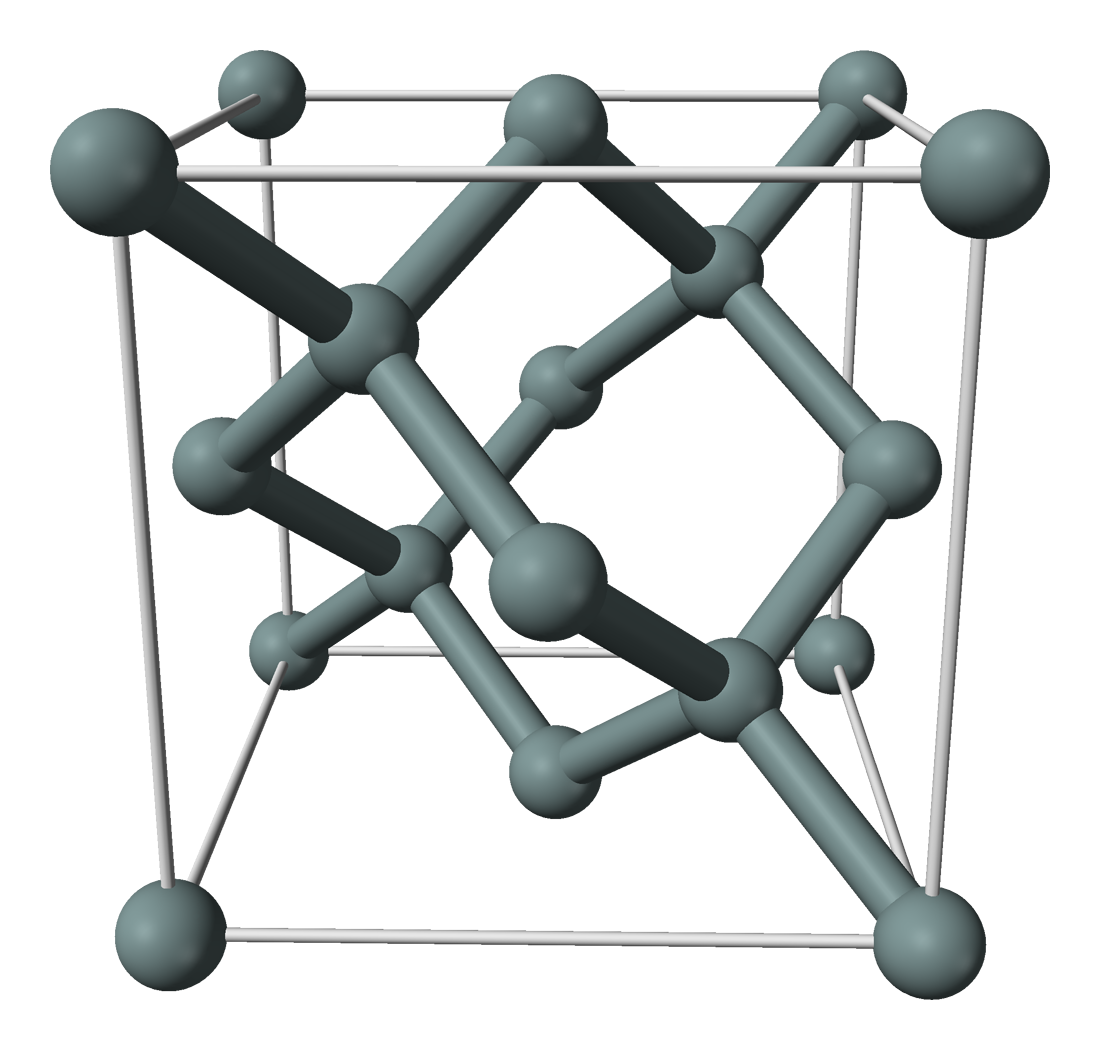
\includegraphics[width=0.5\textwidth,height=0.4\textwidth]{./images/electrical/silicon.png}
\\

\end{tabular}
\caption{Left) Marbles in an ordered arrangement on a solitaire board \cite{image_marbles}; Right) Silicon atoms ordered within a material\cite{image_silicon} Both systems are highly ordered.}
\label{fig:order}
\end{figure}

\begin{figure}[H]
\centering
\begin{tabular}{ c c }



\includegraphics[width=0.5\textwidth,height=0.4\textwidth]{./images/electrical/spaghetti.jpg}

&
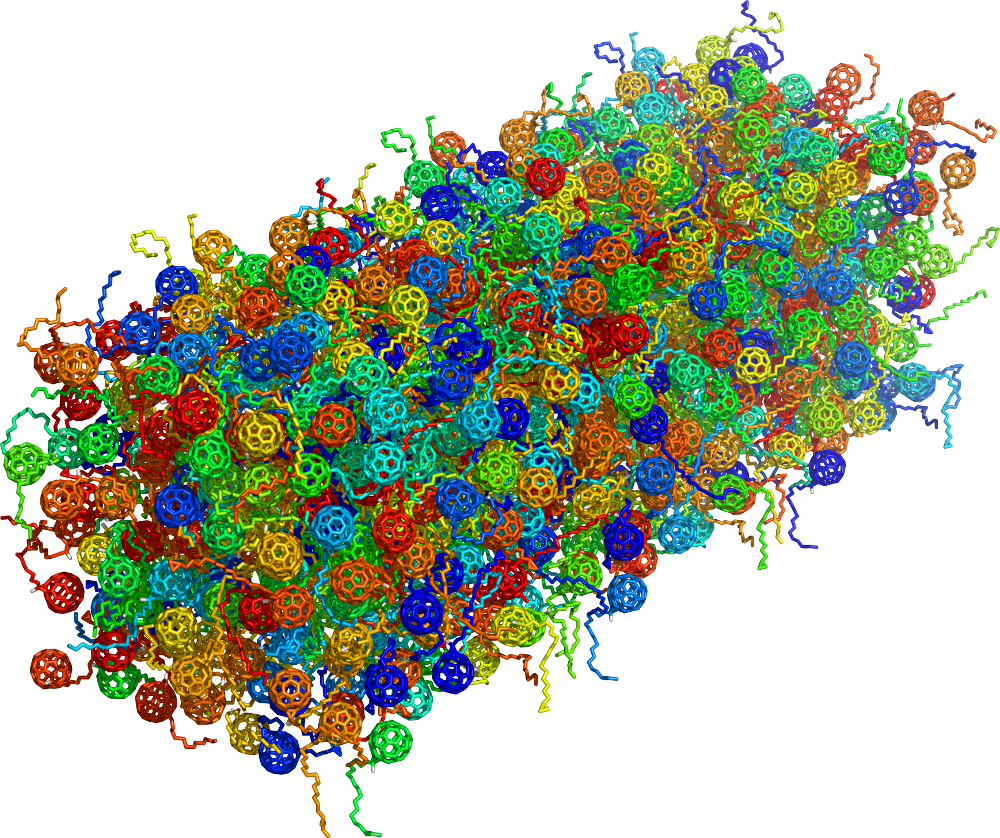
\includegraphics[width=0.5\textwidth,height=0.4\textwidth]{./images/electrical/polymer.png}
\\
\end{tabular}
\caption{Left) A plate of spaghetti \cite{image_spaghetti}; Right) A polymer packing like spaghetti. Both systems are highly disordered.}
\label{fig:disorder}
\end{figure}

So on one hand we have an organic material that is messy and highly disordered, and on the other hand we have a material such as silicon that is highly pure and very ordered.  This physical differences results in a very different energetic landscape for the two materials. In the ordered material semiconductor electrons/holes can travel freely in the conduction and valance bands. If an electric field is applied they only experience a small resistive force. Such a band structure is shown in Figure \ref{fig:band_structure}a. In the organic material the picture is very different, due to the disorder and impurities the band structure is full trap states. There are so many trap states that the carriers no longer move freely but hop between the trap states after being thermally excited, such a band structure is shown in shown in Figure \ref{fig:band_structure}b. Thus there are two very different charge transport mechanisms in these two materials.


\begin{figure}[H]
\centering
\begin{tabular}{ c c }


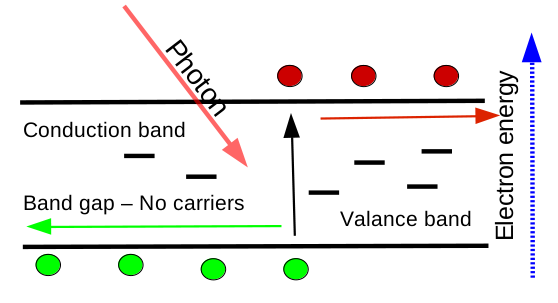
\includegraphics[width=0.5\textwidth,height=0.32\textwidth]{./images/electrical/ordered.png}

&
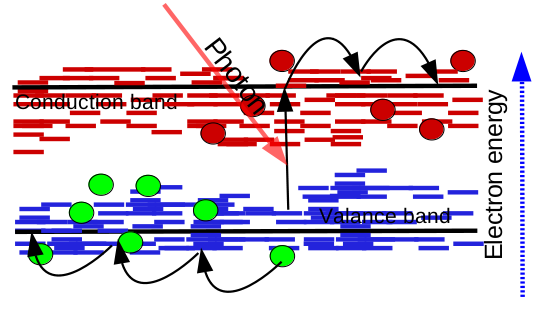
\includegraphics[width=0.5\textwidth,height=0.32\textwidth]{./images/electrical/disordered.png}
\\
\end{tabular}
\caption{a) The band structure of an ordered semiconductor such as GaAs; b) The band structure of an disordered material such as PM6:Y6 or P3HT:PCBM.}
\label{fig:band_structure}
\end{figure}

\subsection{Trap states and charge density}
[This section needs improving/editing but the sketch of what it should say is there:]
Figure \ref{fig:dos_image} sketches out the distribution of states for Figure \ref{fig:band_structure}. On the left of the image is a ordered semiconductor with a parabolic band structure. The Fermi distribution of electrons is coloured in purple. The right hand side image shows a disordered semiconductor with an exponential density of trap states going into the band gap (sometimes a Gaussian DoS is used).  It can be seen that the DoS and the distribution/energetic position of charge carriers are is very different between the two types of semiconductor.


\begin{figure}[H]
\centering
\begin{tabular}{ c c }

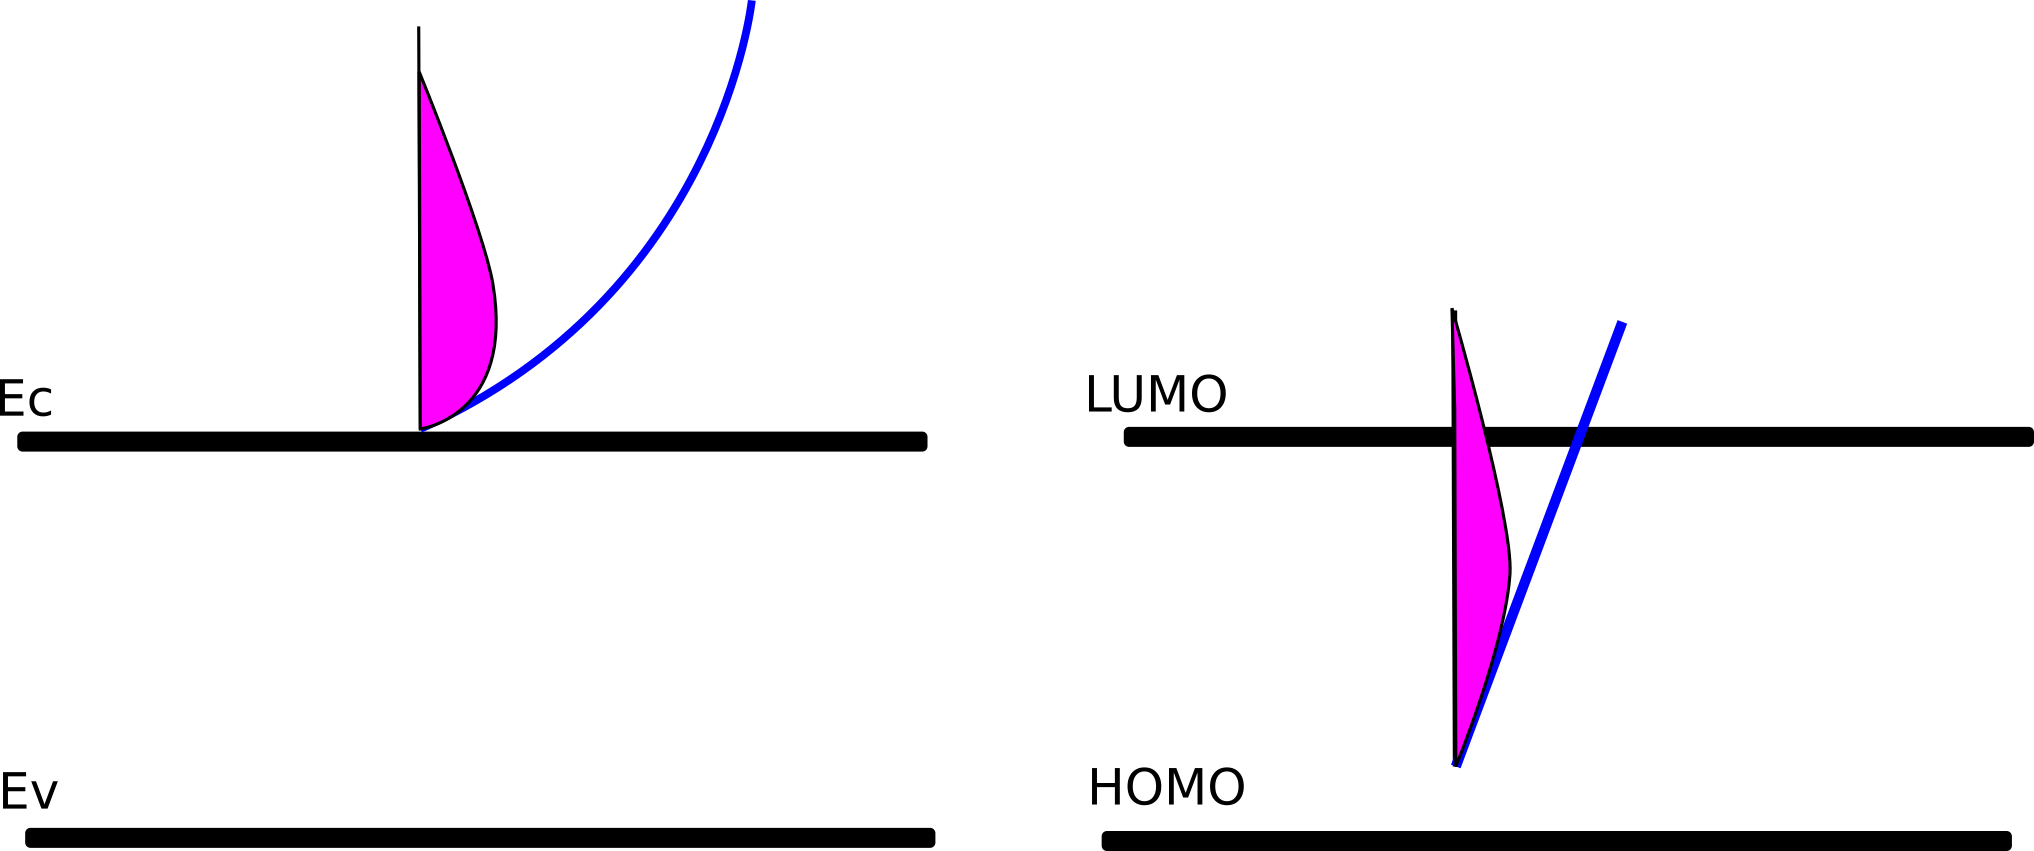
\includegraphics[width=1\textwidth,height=0.4\textwidth]{./images/electrical/band_structure.png}
\\
\end{tabular}
\caption{a) The band structure of an ordered semiconductor such as GaAs; b) The band structure of an disordered material such as PM6:Y6 or P3HT:PCBM.}
\label{fig:dos_image}
\end{figure}

The total charge density at any place in the device can be described by an integration of the Fermi-Dirac function, and the DoS $\rho$.

\begin{equation}
n(E_{f},T)=\int^{\infty}_{E_{min}} \rho(E) f(E,E_{f}) dE
\end{equation}

Where $E_{f}$ is the Fermi level. Clearly $\rho$ will be very different for an ordered and a disordered semiconductor. Thus the dependence of $n(E_{f},T)$ on $E_{f}$ and thus applied voltage will very depending on what $\rho$ is chosen for the device. In practical terms this means that a disordered device will have a lot more traps closer to the Fermi level and thus for any given voltage it will contain one or two orders of magnitude more charge than an ordered device, this can be observed in Charge Extraction experiments. So if one ignores trap states when modelling a disordered device then the function $n(Voltage)$ will be wrong.

If $n(Voltage)$ is not correct then the recombination rate will be wrong for any given voltage:

\begin{equation}
R=k_{r}n(Voltage) p(Voltage)
\end{equation}


Furthermore if $n_{free}(E_{f},T)$ is wrong the mobility will also have an incorrect dependence on voltage:

\begin{equation}
\mu_e(n)=\frac{\mu_e^0 n_{free}}{n_{free}+n_{trap}}
\end{equation}

So if your DoS is wrong (i.e. no traps). Then you have no chance of reproducing a JV curve correctly.  Summary: OghmaNano was written specifically to simulate disordered devices where trap states are play a large role in transport and recombination. Examples of such materials are PM6:Y6 and P3HT:PCBM. OghmaNano includes traps correctly, make sure what ever model you are using also includes traps or it will be wrong.

\subsection{Why you should not use Langevin recombination in device models}
Langevin recombination is defined as,

\begin{equation}
R_{free}=q k_{r}\frac{( \mu_e+ \mu_h) }{2\epsilon_0\epsilon_r} n p
\end{equation}

where $R_{free}$ is the recombination rate, $k_{r}$ is the Langevin reduction factor and all other symbols have their usual meaning. In general Langevin recombination is a bad way to describe recombination in OPV devices. There were some older papers from the early 2010s using this mechanisum but the models could not self consistently describe dark and light JV curves. This is because the mechanism assumes Brownian motion of electrons and holes and that charge carriers of opposite polarity will recombine when they get close enough to fall into each others electrostatic field.  This picture assumes the charge carriers are free and completely neglects the influence of trap states. It was often found that the Langevin equation could not reproduce the experimental results and predicted recombination rates far higher than were experimental observed. To account for this a Langevin reduction factor $k_{r}$ was often introduced into the equation, and a lot of effort went into measuring $k_{r}$. This need for a reduction factor pointed at some deeper issues with the equation.

If we look at the equation for Langevin recombination we can immediately see some issues with it. The first thing we notice is that $R_{free}$ can only ever change as the square of the charge density (n p), but we know from experiment $R_{free}$ can is often a higher order than 2 e.g. $(np)^{1.5}$. Furthermore we can see two mobility terms, however we know from the discussion from above that mobility is a function of carrier density. So the fact that it has the wrong dependence on carrier density and needs a reduction factor points at the mechanism on which it is based being incorrect, and using it will always be like trying to get a square peg in a round hole. 

\subsection{How one can make Langevin recombination work in device models}
So they key problems with Langevin recombination are a wrong dependence on carrier density and the need for a reduction factor. It is possible to make Langevin recombination 'work' by making the charge carrier mobilities a function of carrier density as was done in \cite{mackenzie2011modeling}:

\begin{equation}
R_{free}=q k_{r}\frac{(\alpha \mu_e(n)+\beta \mu_h(n)) n_{tot} p_{tot}}{2\epsilon_0\epsilon_r}
\end{equation}

then by defining a mobility edge and assuming any carrier below the mobility edge could not move and any carrier above it could.  One could define the averaged electron/hole mobility as: 

\begin{equation}
\mu_e(n)=\frac{\mu_e^0 n_{free}}{n_{free}+n_{trap}}
\end{equation}

and

\begin{equation}
\mu_h(n)=\frac{\mu_h^0 p_{free}}{p_{free}+p_{trap}}
\end{equation}

and if one assumes the density of free charge carriers is much smaller than the density of trapped charge carriers one can arrive at

\begin{equation}
R(n,p)=q k_{r}\frac{(\alpha \mu_e^0 n_{free} p_{trap}+\beta \mu_h p_{free} n_{trap}) }{2\epsilon_0\epsilon_r}
\end{equation}

Thus by making the mobility carrier density dependent we arrive at an expression for Langeving recombination that's dependent upon the density of free and trapped carriers (i.e. $n_{free} p_{trap}$ and $ p_{free} n_{trap}$). This is in principle the same as SRH recombination (i.e. a process involving free electrons (holes) recombining with trapped holes (electrons)).  This was a nice simple approach and it worked quite well in the steady state.  However, to make this all work we have to assume all electrons (holes) at any given position in space had a single quasi-Fermi level, which meant they were all in equilibrium with each other.  For this to be true, all electrons (holes) would have to be able to exchange energy with all other electrons (holes) at that position in space and have an infinite charge carrier thermalization velocity.  This is an OK assumption in steady state when electrons (holes) had time to exchange energy, however once we start thinking about things happening in time domain, it becomes harder to justify because there are so many trap states in the device it is unlikely that charge carriers will be able to act as one equilibrated gas with one quasi-Fermi level.  On the other hand the SRH mechanism does not make this assumption, so it is a better description of recombination/trapping.



